\documentclass{lug}

\title{Your Next Linux Notebook for Only \$10}
\subtitle{How to Install Debian on PowerPC}
\author{Jack Rosenthal}
\date{2017-04-13}
\institute{Mines Linux Users Group}

\usepackage{array}

\begin{document}

\begin{frame}{Why am I giving this talk?}
    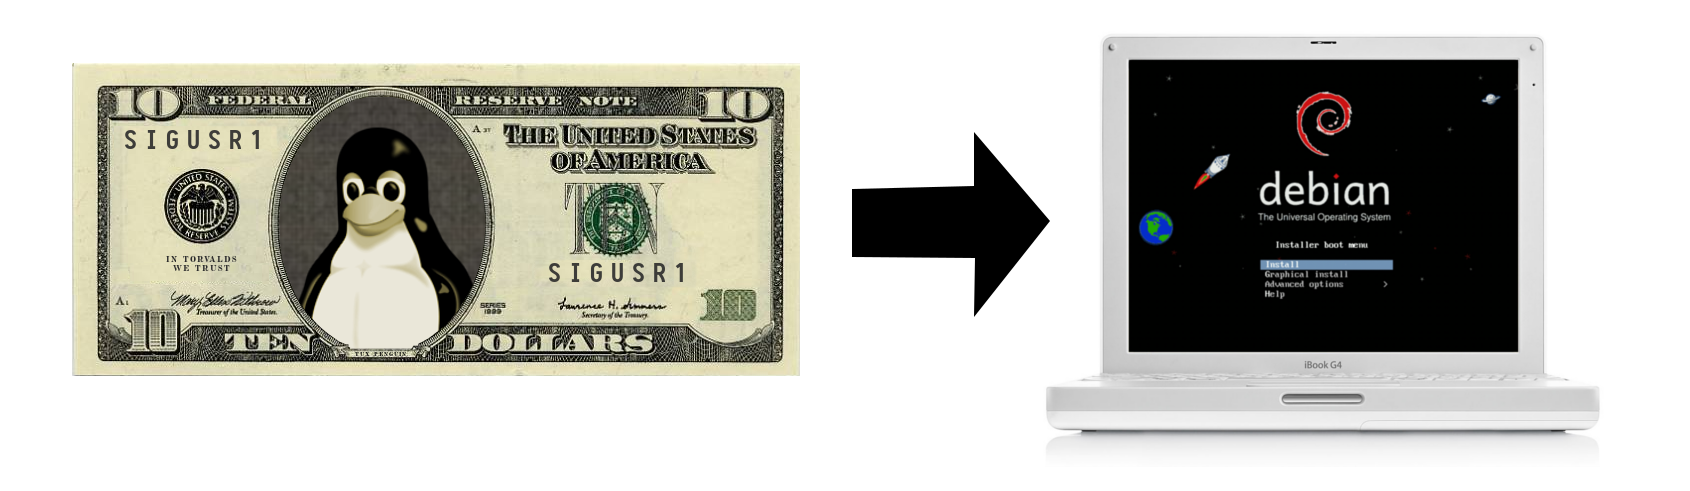
\includegraphics[width=\linewidth]{graphics/10toG4}

    \begin{itemize}[<+->]
        \item To show an inexpensive option for tinkering with Linux on another
            computer
        \item To show Linux will run on nearly anything
        \item \emph{You can have another Linux notebook for less than the cost
            of dinner!}
    \end{itemize}
\end{frame}

\begin{frame}{What options are available?}
    \small

    \begin{tabular}{ >{\centering\arraybackslash}m{0.3\textwidth} >{\centering\arraybackslash}m{0.3\textwidth} >{\centering\arraybackslash}m{0.3\textwidth} }

        \textbf{iBook G3}\par ``Clamshell'' &
        \textbf{iBook G3}\par ``Snow'' &
        \textbf{iBook G4} \\[10pt]

        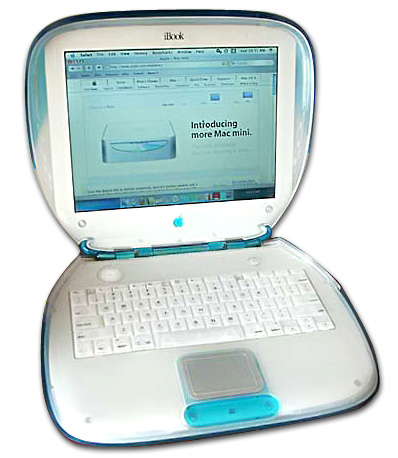
\includegraphics[height=70pt]{graphics/clamshell.jpg} &
        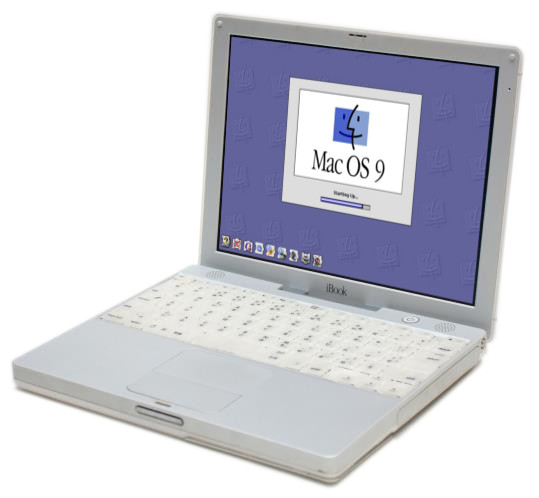
\includegraphics[height=70pt]{graphics/ibooksnow.jpg} &
        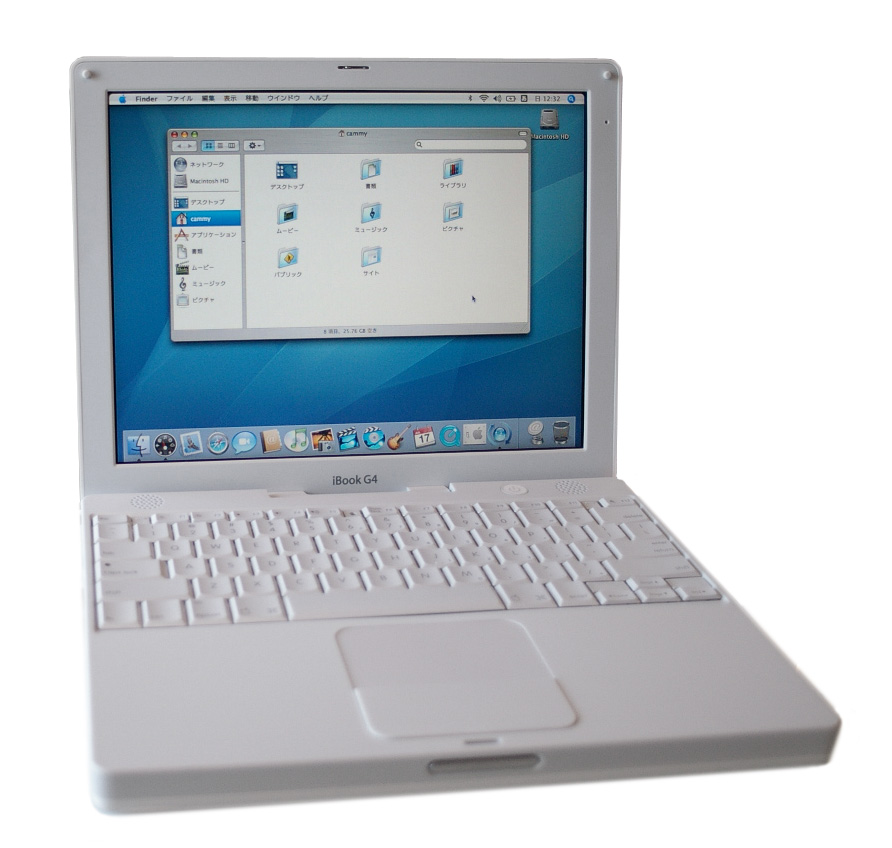
\includegraphics[height=70pt]{graphics/g4.jpg} \\
    \end{tabular}

    \pause

    \scriptsize
    \begin{tabular}{ p{0.3\textwidth} p{0.3\textwidth} p{0.3\textwidth} }
         300 MHz -- 466 MHz        & 500 MHz -- 900 MHz      & 800 MHz -- 1.42 GHz      \\
         Max 576 MB RAM            & Max 640 MB RAM          & Max 1.5 GB RAM           \\
         800x600 12"               & 1024x768 12.1" or 14.1" & 1024x768 12.1" or 14.1"  \\
         CD-ROM (Tray)             & CD or DVD (Tray)        & DVD (Slot)               \\
         Mac OS 8.6 or 9           & Mac OS 9                & No Mac OS Support        \\
         Mac OS X (up to 10.4)     & Mac OS X (up to 10.4)   & Mac OS X (up to 10.5)    \\
         Repairability: 4/5        & Repairability: 0/5      & Repairability: -1/5      \\
         Expect to pay \$60--\$200 & Expect to pay \$5--\$30 & Expect to pay \$10--\$40 \\
    \end{tabular}

    \pause

    \begin{center}
        \small
        \textbf{Other Options?} Any 2000's PowerBook
    \end{center}

\end{frame}

\begin{frame}{How Install Debian?}
    \begin{columns}
        \begin{column}{0.7\textwidth}
            \begin{enumerate}
                \setlength\itemsep{1em}
                \item Download Debian PowerPC ISO from \url{https://debian.org}
                \item Burn it to a CD
                \item Put in iBook
                \item Hold C-key while booting
                \item Install using pretty interface
                \item \dots
                \item Profit?
            \end{enumerate}
        \end{column}
        \begin{column}{0.3\textwidth}
            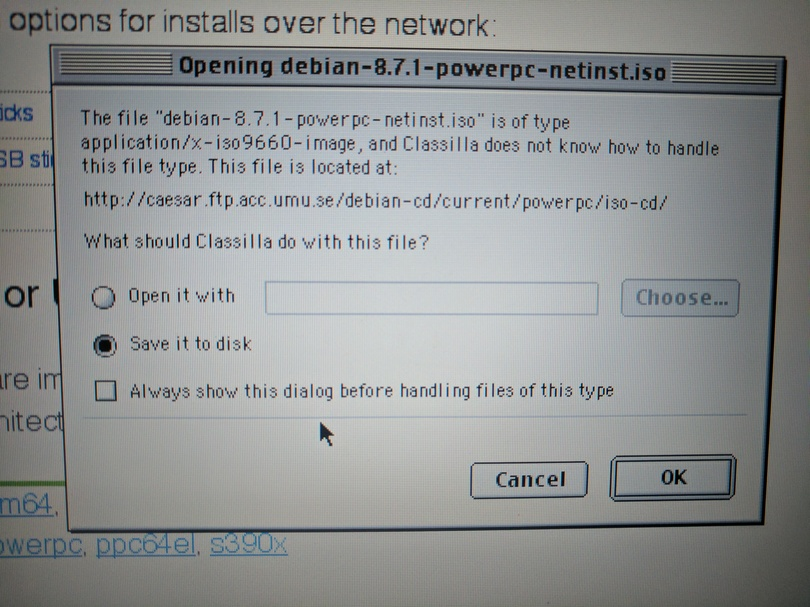
\includegraphics[width=\textwidth]{graphics/download}\par
            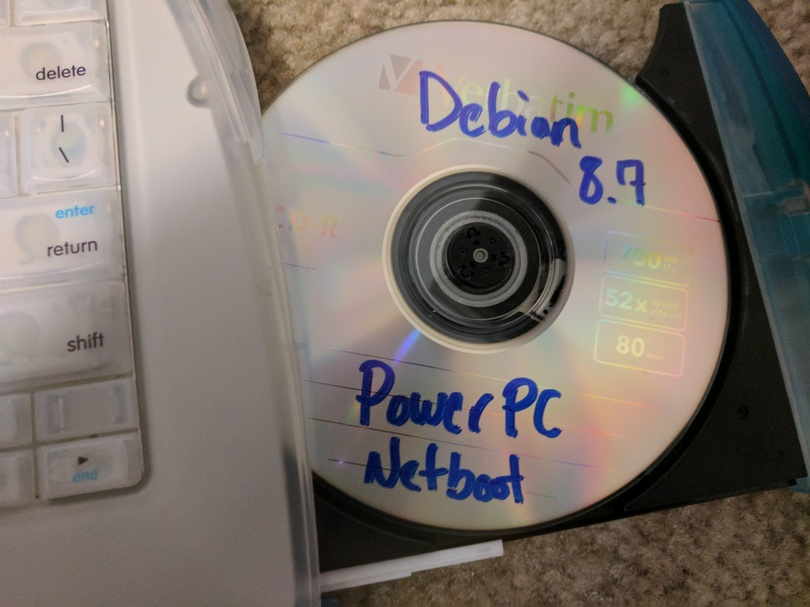
\includegraphics[width=\textwidth]{graphics/cd}\par
            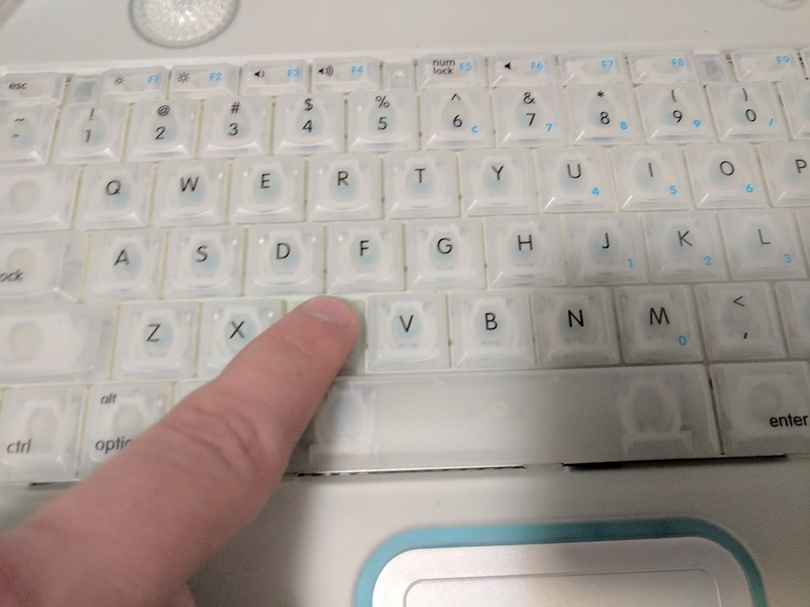
\includegraphics[width=\textwidth]{graphics/ckey}\par
        \end{column}
    \end{columns}
\end{frame}

\begin{frame}{Profit? Not quite yet.}
    \begin{itemize}[<+->]
        \setlength\itemsep{1em}
        \item Tweak the graphics to work better\par
            {\small I found the \texttt{radeon.agpmode=-1} kernel flag makes my
            iBook G4 happy}
        \item Install wireless firmware\par
            {\small Either the \texttt{firmware-b43-installer} or
            \texttt{firmware-b43legacy-installer} package}
        \item The touchpad is an ADB mouse, and you will probably want to
            emulate right/middle click using keyboard keys. Edit
            \texttt{/etc/defaults/mouseemu} to configure.
        \item Can anyone figure out how to get battery display working? If so,
            I will update the slides.
    \end{itemize}
\end{frame}

\begin{frame}{yaboot}
    Debian installs yaboot, a bootloader that works on OpenFirmware. Out of the
    box, it works fine. But you may wish to tweak it.
    \pause
    \begin{itemize}[<+->]
        \item Configured in \texttt{/etc/yaboot.conf}
        \item Adjust \texttt{timeout=} to your liking (potentially \texttt{0})
        \item Add any kernel flags you need with \texttt{append=}
        \item Run \texttt{ybin} as root to regenerate the bootloader and bless
            it with Holy Penguin Pee
    \end{itemize}
\end{frame}

\begin{frame}{Other Options for Linux on an iBook?}
    \begin{itemize}[<+->]
        \item Ubuntu maintains a PowerPC release
        \item Gentoo is available for PowerPC
        \item Build Linux from source
        \item *BSD
    \end{itemize}
\end{frame}

\begin{frame}
    \centering
    \Huge
    Questions?
\end{frame}

\end{document}
